\documentclass[dvipdfmx,12pt]{standalone}
\standaloneconfig{class=beamer}

%%%% Tikz環境 %%%%
\usepackage{tikz}
\usetikzlibrary{calc,decorations.pathreplacing,quotes,positioning,shapes,fit,arrows,backgrounds,tikzmark}
%%%%%%%%

\tikzset{
	pvebnode/.pic={
		\node(-summary) [fill=orange, minimum size = 1em] at (0,0) {};
		\node(-cluster) [fill=green, minimum size = 1em, left=of -summary]{};
		\draw[pic actions] ($(-cluster.east)+(.5,-.5)$) rectangle ($(-summary.west)+(-.5,.5)$);
	}
}

\begin{document}
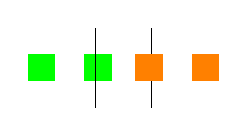
\begin{tikzpicture}
	\pic[fill=blue!10] (a1) {pvebnode};
	\pic[fill=red!10, left=1em of a1-summary.west] (a2) {pvebnode};
	%\draw 


\end{tikzpicture}
\end{document}
